% AQNet mathematical analysis, part 1 of 4.
% Required packages in main.tex: amsmath, amssymb, booktabs, graphicx, tikz.
\section{Queuing Model and Assumptions}
\label{sec:b1_queuing}

AQNet (Asynchronous Queuing Network Simulator) represents a multi-hop
packet-switched network with non-blocking store-and-forward operations.
A node receives a packet, stores it if necessary, and schedules later
processing rather than synchronously waiting for forwarding to finish.
The queuing model provides a mathematical abstraction of that behaviour.

\subsection{Queuing Models Used in AQNet}
Table~\ref{tab:b1_nodes} summarises six queuing models and their
interpretation in AQNet. The M/M/1 model provides an isolated
baseline rather than an additional network node.

\begin{table}[htbp]
\centering
\small
\caption{Queuing models and their roles in AQNet}
\label{tab:b1_nodes}
\begin{tabular}{@{}lp{0.65\linewidth}@{}}
\toprule
Model & Interpretation in AQNet \\
\midrule
M/M/1 & One output port with an effectively unlimited waiting queue (baseline). \\
M/M/1/K & Edge router N1 with one server and finite system capacity. \\
M/M/$\infty$ & Propagation stage L1 with no contention for servers. \\
M/M/n/n & N3: $n$ service channels, no waiting room; reject if all are busy. \\
M/M/c & N4: $c$ service channels with a shared waiting queue. \\
M/M/c/K & N2: $c$ service channels with finite system capacity. \\
\bottomrule
\end{tabular}
\end{table}

\subsection{Notation and Model Assumptions}
Let $\lambda_i$ denote the mean packet arrival-attempt rate at node $i$
(packets/s), $\mu_i$ the mean service rate of one server (packets/s),
$c_i$ the number of identical servers, and $K_i$ the maximum number
of packets in the node, including those in service. The mean service
time is $1/\mu_i$. A finite-server offered-load ratio is
\begin{equation}
\rho_i=\frac{\lambda_i}{c_i\mu_i},
\qquad a_i=\frac{\lambda_i}{\mu_i}.
\label{eq:b1_load}
\end{equation}
For one server, $c_i=1$. For M/M/$\infty$, $a_i$ is an offered load,
not a finite-server utilisation ratio.

The isolated M/M formulas assume Poisson arrival attempts and
exponentially distributed service times. FCFS and a common waiting
queue are assumed for multi-server waiting models. These are
\emph{analytical assumptions}, not claims about every traffic stream
inside the coupled AQNet network. In particular, a finite buffer or
TTL expiration can alter traffic seen by downstream nodes. Throughout the analysis, $K_i$ denotes total system capacity,
including service positions; this convention must also be used
when interpreting simulation results.

% AQNet mathematical analysis, part 2 of 4.
\section{AQNet Topology and Network Equations}
\label{sec:b2_aqnet}

\subsection{Network Topology}
The network configuration considered in this analysis consists of SRC $\to$ N1 $\to$ L1
$\to$ N2. A packet forwarded from N2 goes to N3 with probability
$0.6$ or to N4 with probability $0.4$, and then reaches SNK if
successfully delivered (Figure~\ref{fig:b2_aqnet}). An isolated
M/M/1 system is used separately as a baseline.

\begin{figure}[htbp]
\centering
\resizebox{\linewidth}{!}{%
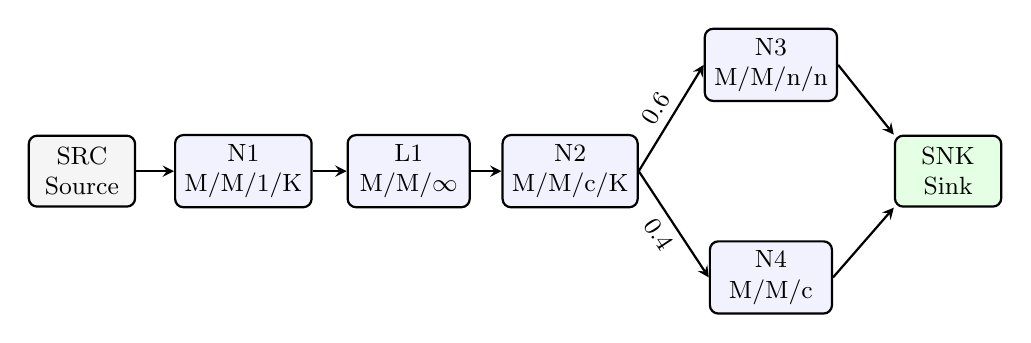
\begin{tikzpicture}[>=stealth,
    every node/.style={font=\small},
    queue/.style={draw,rounded corners=3pt,thick,minimum width=1.55cm,
        minimum height=0.9cm,align=center,fill=blue!5},
    endpoint/.style={draw,rounded corners=3pt,thick,
        minimum width=1.35cm,minimum height=0.9cm,align=center}]
\node[endpoint,fill=gray!8] (src) at (0,0) {SRC\\Source};
\node[queue] (n1) at (2.05,0) {N1\\M/M/1/K};
\node[queue] (l1) at (4.15,0) {L1\\M/M/$\infty$};
\node[queue] (n2) at (6.2,0) {N2\\M/M/c/K};
\node[queue] (n3) at (8.75,1.35) {N3\\M/M/n/n};
\node[queue] (n4) at (8.75,-1.35) {N4\\M/M/c};
\node[endpoint,fill=green!10] (snk) at (11.0,0) {SNK\\Sink};
\draw[->,thick] (src) -- (n1);
\draw[->,thick] (n1) -- (l1);
\draw[->,thick] (l1) -- (n2);
\draw[->,thick] (n2.east) -- node[above,sloped] {$0.6$} (n3.west);
\draw[->,thick] (n2.east) -- node[below,sloped] {$0.4$} (n4.west);
\draw[->,thick] (n3.east) -- (snk.north west);
\draw[->,thick] (n4.east) -- (snk.south west);
\end{tikzpicture}%
}
\caption{AQNet network model and routing probabilities.}
\label{fig:b2_aqnet}
\end{figure}

Figure~\ref{fig:b2_aqnet} represents the feed-forward configuration
used in this analysis. Node-specific parameters are defined separately,
and feedback links are not included in this configuration.

\subsection{Traffic Flow Equations}
For an ideal lossless open network, the standard flow equation is
\begin{equation}
\lambda_i=\gamma_i+\sum_j\lambda_jp_{ji},
\label{eq:b2_ideal_flow}
\end{equation}
where $\gamma_i$ is the external arrival rate and $p_{ji}$ is the
routing probability from node $j$ to node $i$.

For a network with rejection, distinguish the \emph{offered rate}
$\lambda_i$ from the \emph{successful forwarding rate} $X_i$:
\begin{equation}
\lambda_i=\gamma_i+\sum_j X_jp_{ji}.
\label{eq:b2_actual_flow}
\end{equation}
For the feed-forward AQNet configuration this becomes
\begin{align}
\lambda_{N1}&=\lambda_{\mathrm{SRC}}, &
\lambda_{L1}&=X_{N1},\\
\lambda_{N2}&=X_{L1}, &
\lambda_{N3}&=0.6X_{N2},\\
\lambda_{N4}&=0.4X_{N2}, &
X_{\mathrm{SNK}}&=X_{N3}+X_{N4}.
\label{eq:b2_node_flows}
\end{align}
These equalities assume that successful downstream forwarding follows
the illustrated routes and that packets are not duplicated.
Additional routes or feedback links require additional flow terms.

% AQNet mathematical analysis, part 3 of 4.
\subsection{Admission, Blocking and Stability}
Let $P_{\mathrm{block},i}$ be the probability that a packet offered to
node $i$ is rejected for lack of capacity. The admitted rate is
\begin{equation}
\lambda_{\mathrm{eff},i}=\lambda_i(1-P_{\mathrm{block},i}).
\label{eq:b2_admitted}
\end{equation}
If all admitted packets complete service without further failures,
$X_i=\lambda_{\mathrm{eff},i}$. If packets expire or fail after admission,
then $X_i$ may be smaller. Under the isolated Poisson-arrival
assumptions, M/M/1/K and M/M/c/K have
$P_{\mathrm{block}}=p_K$, while M/M/n/n uses Erlang B:
\begin{equation}
P_{\mathrm{block}}=\frac{a^n/n!}{\displaystyle\sum_{k=0}^{n}a^k/k!},
\qquad a=\lambda/\mu.
\label{eq:b2_erlang_b}
\end{equation}
These are not automatically exact for downstream AQNet traffic altered
by earlier packet losses.

For infinite-waiting-room M/M/1 and M/M/c models, the familiar
steady-state conditions are, respectively,
\begin{equation}
\lambda<\mu,
\qquad\lambda<c\mu\quad\text{(M/M/c)}.
\label{eq:b2_stability}
\end{equation}
Thus the M/M/c node N4 requires
$\lambda_{N4}<c_{N4}\mu_{N4}$ under its model assumptions. Finite
systems N1, N2 and N3 have bounded occupancy and can have a
stationary distribution even at offered load ratios of one or above,
although blocking may become substantial. The ideal M/M/$\infty$
stage has no server-contention waiting.

\subsection{End-to-End Delay}
For a packet $k$ successfully delivered from SRC to SNK, define
\begin{equation}
D_k=t_{k,\mathrm{SNK}}-t_{k,\mathrm{SRC}}.
\label{eq:b2_packet_delay}
\end{equation}
The reported mean is calculated over successful deliveries:
\begin{equation}
D_{\mathrm{E2E}}=\frac{1}{N_{\mathrm{success}}}
\sum_{k\in\mathcal{S}}D_k,\quad
N_{\mathrm{success}}=|\mathcal{S}|>0.
\label{eq:b2_mean_delay}
\end{equation}

For a simplified \emph{lossless} path calculation, let $W_i$ be the
mean sojourn time at node $i$. The two possible paths have
\begin{align}
D_3&=W_{N1}+W_{L1}+W_{N2}+W_{N3},\\
D_4&=W_{N1}+W_{L1}+W_{N2}+W_{N4}.
\end{align}
If successful deliveries retain the routing proportions, their mean is
\begin{equation}
D_{\mathrm{E2E}}=0.6D_3+0.4D_4.
\label{eq:b2_path_mean}
\end{equation}
With unequal branch success probabilities $g_3,g_4$, the routing
weights must instead be conditioned on successful delivery:
\begin{equation}
q_3=\frac{0.6g_3}{0.6g_3+0.4g_4},\quad q_4=1-q_3,
\label{eq:b2_conditional_weights}
\end{equation}
provided the denominator is nonzero. The corresponding mean is
$q_3D_{3|\mathrm{success}}+q_4D_{4|\mathrm{success}}$.

% AQNet mathematical analysis, part 4 of 4.
\subsection{Analytical Validity and Jackson Network Limitations}
The classical open Jackson network provides a product-form
steady-state solution under its specified assumptions. The AQNet model additionally includes finite-capacity rejection and
potential TTL/timeout termination. These can change downstream arrival
streams and create dependencies between nodes. Therefore the classical
Jackson product-form solution must \emph{not} be assumed exact for
AQNet as a whole. Isolated-node M/M formulas remain analytical
references only when their individual assumptions apply.

A full buffer may cause packet dropping or upstream backpressure,
depending on the forwarding mechanism. The blocking equations above
represent admission rejection, whereas a backpressure model requires
additional treatment of upstream dependencies. The M/M/$\infty$ stage
idealises propagation using exponential service times and no
server contention, rather than an exact physical link-delay model.

\subsection{Model Consistency Conditions}
The following conditions support consistency checks between the
mathematical model and simulation results:
\begin{align}
&p_{N2,N3}+p_{N2,N4}=0.6+0.4=1,
\label{eq:b2_routing_sum}\\
&0\leq N_i(t)\leq K_i\quad\text{(finite-capacity node)},
\label{eq:b2_capacity}\\
&L_i=\lambda_{\mathrm{eff},i}W_i
\quad\text{(consistent steady-state population)}.
\label{eq:b2_little}
\end{align}
Packet outcomes should also be counted without overlap:
\begin{equation}
\begin{split}
N_{\mathrm{generated}}={}&N_{\mathrm{delivered}}+
N_{\mathrm{rejected}}\\
&+N_{\mathrm{terminated}}+N_{\mathrm{remaining}}.
\end{split}
\label{eq:b2_balance}
\end{equation}
The conservation check assumes every generated packet appears in
exactly one final status category at the observation end. Little's
Law also requires consistent arrival/exit populations, especially if
packets terminate after admission.

\subsection{Scope of the Analytical Model}
The equations describe the feed-forward routing configuration in
Figure~\ref{fig:b2_aqnet}, with $K_i$ defined as total capacity.
Node-specific arrival and service parameters determine numerical
performance estimates. TTL expiration is treated as a separate
packet-termination outcome; its threshold and triggering rule are
model parameters. The formulas are analytical relationships, not
measured network results.
